\documentclass[a4paper,12pt,twoside,openright,titlepage]{book}

%Additional packages
\usepackage[ascii]{inputenc}
\usepackage[T1]{fontenc}
\usepackage[dutch,english]{babel}
\usepackage{imakeidx}
\usepackage{syntonly}
\usepackage[official]{eurosym}
%\usepackage[graphicx]
\usepackage{graphicx}
\graphicspath{ {./images/} }
\usepackage{float}
\usepackage{hyperref}
\hypersetup{colorlinks=true, linkcolor=blue, citecolor=blue, filecolor=blue, urlcolor=blue, pdftitle=, pdfauthor=, pdfsubject=, pdfkeywords=}
\usepackage{tabularx}
\usepackage{scrextend}
\addtokomafont{labelinglabel}{\sffamily}
\usepackage{listings}
\usepackage{adjustbox}
\usepackage{color}

% Define colors
\definecolor{ashgrey}{rgb}{0.7, 0.75, 0.71}

% Listing style
\lstset{
  backgroundcolor=\color{ashgrey},   % choose the background color; you must add \usepackage{color} or \usepackage{xcolor}; should come as last argument
  basicstyle=\footnotesize,        % the size of the fonts that are used for the code
  breakatwhitespace=false,         % sets if automatic breaks should only happen at whitespace
  breaklines=true,                 % sets automatic line breaking
  extendedchars=true,              % lets you use non-ASCII characters; for 8-bits encodings only, does not work with UTF-8
  frame=single,	                   % adds a frame around the code
  keepspaces=true,                 % keeps spaces in text, useful for keeping indentation of code (possibly needs columns=flexible)
  rulecolor=\color{black},         % if not set, the frame-color may be changed on line-breaks within not-black text (e.g. comments (green here))
  showspaces=false,                % show spaces everywhere adding particular underscores; it overrides 'showstringspaces'
}

% Uncomment for production
% \syntaxonly

% Style
\pagestyle{headings}

% Turn on indexing
\makeindex

% Define document
\author{D. Leeuw}
\title{Linux deel 3: Server}
%\subtitle{Linux voor MBO niveau 4 en het LPI Linux Essentials examen}
%\subject{Een Praktische Gids}
\date{\today\\v.0.1.0}

\begin{document}
\selectlanguage{dutch}

\maketitle

\copyright\ 2021 Dennis Leeuw\\

\begin{figure}

\includegraphics[width=0.3\textwidth]{CC-BY-SA-NC.png}
\end{figure}

\bigskip

Dit werk is uitgegeven onder de Creative Commons BY-NC-SA Licentie en laat anderen toe het werk te kopi\"eren, distribueren, vertonen, op te voeren, en om afgeleid materiaal te maken, zolang de auteurs en uitgever worden vermeld als maker van het werk, het werk niet commercieel gebruikt wordt en afgeleide werken onder identieke voorwaarden worden verspreid.


%%%%%%%%%%%%%%%%%%%
%%% Introductie %%%
%%%%%%%%%%%%%%%%%%%

\frontmatter
\chapter{Over dit Document}
Dit document behandeld Linux voor het middelbaar beroepsonderwijs in Nederland, maar kan breder ingezet worden, daar het gericht is op het behalen van het LPI Linux Essentials examen. De doelgroep is niveau 4 van het MBO, met enige kennis van computers.

\section*{Versienummering}
Het versienummer van elk document bestaat uit drie nummers gescheiden door een punt. Het eerste nummer is het major-versie nummer, het tweede nummer het minor-versienummer en de laatste is de nummering voor bug-fixes.\par
Om met de laatste te beginnen als er in het document slechts verbeteringen zijn aangebracht die te maken hebben met type-fouten, websites die niet meer beschikbaar zijn, of kleine foutjes in de opdrachten dan zal dit nummer opgehoogd worden. Als docent of student hoef je boek niet te vervangen. Het is wel handig om de wijzigingen bij te houden.\par
Als er flink is geschreven aan het document dan zal het minor-nummer opgehoogd worden, dit betekent dat er bijvoorbeeld plaatjes zijn vervangen of geplaatst/weggehaald, maar ook dat paragrafen zijn herschreven, verwijderd of toegevoegd, zonder dat de daadwerkelijk context is veranderd. Een nieuw cohort wordt aangeraden om met deze nieuwe versie te beginnen, bestaande cohorten kunnen doorwerken met het boek dat ze al hebben.\par
Als het major-nummer wijzigt dan betekent dat dat de inhoud van het boek substantieel is gewijzigd om bijvoorbeeld te voldoen aan een nieuw kwalificatiedossier voor het onderwijs of een nieuwe versie van Linux Essentials van de LPI. Een nieuw major-nummer betekent bijna altijd voor het onderwijs dat in het nieuwe schooljaar men met deze nieuwe versie aan de slag zou moeten gaan. Voorgaande versies van het document zullen nog tot het einde een schooljaar onderhouden worden, maar daarna niet meer.

\section*{Document ontwikkeling}
Het doel is door middel van open documentatie een document aan te bieden aan zowel studenten als docenten, zonder dat hier hoge kosten aan verbonden zijn en met de gedachte dat we samen meer weten dan alleen. Door samen te werken kunnen we meer bereiken.\par
Bijdragen aan dit document worden dan ook met alle liefde ontvangen. Let u er wel op dat materiaal dat u bijdraagt onder de CC BY-NC-SA licentie vrijgegeven mag worden, dus alleen origineel materiaal of materiaal dat al vrijgegeven is onder deze licentie.\par
De eerste versie is geschreven voor het ROC Horizon College.

\begin{flushleft}
\begin{table}[h!]
\centering
\begin{tabularx}{\textwidth}{ |c|c|c|X| }
\hline
	Versienummer &
	Auteurs &
	Verspreiding &
	Wijzigingen\\
\hline
	0.1.0 &
	Dennis Leeuw &
	Wim Onrust &
	Initieel document\\
\hline
	0.2.0 &
	Dennis Leeuw &
	HEITO18IB-A &
	Toegevoegd: versienummering, de shell, begin van werken met bestanden\\
\hline
\end{tabularx}
\caption{Document wijzigingen}
\label{table:1}
\end{table}
\end{flushleft}



%%%%%%%%%%%%%%%%%
%%% De inhoud %%%
%%%%%%%%%%%%%%%%%
\tableofcontents

\mainmatter
\chapter{Inleiding}
Deze Linux cursus beoogt aan te sluiten bij het Linux Essentials examen van de LPI (Linux Professional Institute). Het boek bestaat uit twee delen in het eerste deel installeren we CentOS als werkstation en leren we het Linux systeem kennen. In het tweede deel installeren we Debian en zullen we meer leren over Linux als server en de interactie tussen Linux systemen.\par
De beide Linux systemen zullen ge\"installeerd worden als virtuele machines op Virtual Box (\url{https://www.virtualbox.org/}). Door gebruik te maken van virtuele machines maakt het onderliggende systeem voor deze cursus niet veel uit en het mag dan ook Windows, Mac OS X of Linux zijn. Voor de CentOS machine is 15G vrije schijfruimte nodig en voor het Debian systeem 8G. Voor elke machine hebben we 2G RAM nodig, dus een totaal van 4G moet vrij beschikbaar zijn.


\chapter{Debian installatie}
%Management netwerk

\chapter{Remote access}
%alleen vanaf het management netwerk

\chapter{Werken met daemons}
\section{init en systemd}

\chapter{Mailserver}
\section{postfix}

\chapter{LAMP}
\section{Apache}
De meest bekende webserver in gebruik op het Internet is de Apache webserver.

Sinds enige tijd is er een webserver die populairder is dan Apache en dat is NGINX die voornamelijk gebruikt wordt in situaties waar performance belangrijk is.

\begin{lstlisting}[language=bash]
$ sudo apt-get install apache2
\end{lstlisting}


\section{MariaDB}
\begin{lstlisting}[language=bash]
$ sudo apt-get install mariadb-server mariadb-client
\end{lstlisting}


\section{PHP}
\begin{lstlisting}[language=bash]
$ sudo apt-get install php
\end{lstlisting}



\chapter{NextCloud}
Je mobiele telefoon synchroniseert zijn data met de cloud. De meeste cloud oplossingen draaien op Linux, maar wat is dat nu eigenlijk; de cloud? Letterlijk betekent cloud wolk en dat is ook waar de term vandaan komt, in tekeningen van computer netwerken wordt een totaal netwerk vaak vervangen door een wolkje. Zoals bijvoorbeeld het Internet.

\begin{figure}
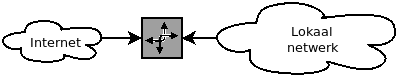
\includegraphics[width=0.99\linewidth]{Cloud_Internet.png}
\end{figure}

De cloud gaat dan ook over diensten die aangeboden worden in een netwerk waarbij het niet meer van belang is op welke machine de data staat, de data bevindt zich ergens in de wolk. Natuurlijk zijn er op de achtergrond fysieke machines waarop de data terecht komt en die beheert moeten worden. In dit hoofdstuk gaan we een machine inrichten met NextCloud. NextCloud is een stukje software geschreven in PHP dat je de mogelijkheid geeft om thuis een cloud systeem te bouwen. Het kan draaien op \'e\'en server met een paar gebruikers en lijkt dan ook heel erg op een NAS (Network Attached Storage) of je kan er een complete cloud dienst mee ontwikkelen dat 100K+ gebruikers ondersteunt zodat het werkt als DropBox of Google Drive. Wij zullen een simpele installatie doen op een enkele (virtuele) machine.

Een NAS gebruikt meestal FTP of SMB om bestanden te delen, Cloud systemen gebruiken het HTTP(s) protocol om via bijvoorbeeld WebDAV data te delen. Dat hoeven niet alleen bestanden te zijn, dat kan ook calender informatie (CalDAV) of adresgegevens (CardDAV) zijn. Met NextCloud zou je je telefoon dus volledig kunnen synchroniseren met je eigen server inplaats van met Google\texttrademark\ of Apple\texttrademark.

NextCloud is een voortzetting van het ownCloud project. De ontwikkeling van ownCloud begon in 2010 en het ownCloud bedrijf ownCloud Inc. werd in 2011 opgericht door Markus Rex, Holger Dyroff and Frank Karlitschek. Het project was bedoelt als een open source vervanger van DropBox. In 2016 werd de code van ownCloud door Frank Karlitschek geforked en omgedoopt tot NextCloud. Een belangrijk deel van het ownCloud ontwikkelteam ging mee met Frank. Sinds 2017 groeit de aanhang van NextCloud, terwijl die van ownCloud daalt.

\section{NextCloud installatie}
In het vorige hoofdstuk heb je al kennis gemaakt met LAMP (Linux, Apache, MySQL en PHP), daar gaan we nu verder mee werken. We gaan MySQL vullen met de gegevens die nodig zijn voor NextCloud en we installeren de NextCloud software, wat PHP is, binnen de Apache omgeving. Om te kunnen beginnen moeten we eerst NextCloud downloaden of installeren vanuit de package manager. Niet elke distributie levert NextCloud mee en omdat het belangrijk is dat je een NextCloud systeem goed bij houdt met betrekking tot de security-patches is het aan te raden om de software zelf te downloaden vanaf de website van NextCloud.

Ga naar \url{https://nextcloud.com/} en klik op Get NextCloud en selecteer Download for Server. Op het moment van schrijven is de meest recente versie versie 19.0.1, dus dat versienummer wordt in de rest van dit document gebruikt. Kijk zelf op de pagina van de NextCloud site wat de meest recente versie is en gebruik dat versienummer in de volgende commando's.

\begin{lstlisting}[language=bash]
$ sudo mkdir -p /srv/www/
$ cd /srv/www/
$ sudo wget https://download.nextcloud.com/server/releases/nextcloud-19.0.1.tar.bz2
$ sudo tar jxvf nextcloud-19.0.1.tar.bz2
\end{lstlisting}

Volg verder de aanwijzingen uit het NextCloud installatie document op \url{https://docs.nextcloud.com/server/19/admin_manual/installation/source_installation.html}.


Voeg de extra PHP modules toe die nodig zijn voor NextCloud
\begin{lstlisting}[language=bash]
$ sudo apt-get install php-curl php-gd php-mbstring php-intl php7.3-mysql php7.3-xml php-zip php-bz2
\end{lstlisting}


%%%%%%%%%%%%%%%%%%%%%
%%% Index and End %%%
%%%%%%%%%%%%%%%%%%%%%
\backmatter
\printindex
\end{document}

%%% Last line %%%
